%%%%%%%%%%%%%%%%%%%%%%%%%%%%%%%%%%%%%%%%%%
% Master Thesis 
% Polina Polunina
% October 2022 
%
% License:
% CC-BY-SA 4.0 -- Creative Commons Attribution-ShareAlike 4.0 International
% https://creativecommons.org/licenses/by-sa/4.0/legalcode
%%%%%%%%%%%%%%%%%%%%%%%%%%%%%%%%%%%%%%%%%%
\section{Methods} \label{sec:methods}
In the following sections, the technical details of the methods used within the thesis will be discussed. First, an evaluation of needs, including currently available data, will be described in \cref{sec:methods:needs}, followed by an explanation of existing Galaxy workflows in \cref{sec:methods:existing}. Then, \cref{sec:methods:changes} will discuss improvements of existing steps in these workflows and the addition of new steps. The following \cref{sec:methods:evaluation} will expose metrics for the evaluation of workflows and the characteristics of their comparison to other methods. Particularly, \cref{sec:methods:evaluation:mock} will give details of benchmarking with regard to the other state-of-the-art approach. Then, \cref{sec:methods:evaluation:real} will give an explanation of benchmarking results produced by both workflows on chosen real-world datasets.

    \subsection{Workflow reengineering} 
        \subsubsection{Evaluation of the needs} \label{sec:methods:needs}
            \paragraph{Characteristics to be considered for improvement}
            The purpose of this master thesis is to create Galaxy workflows to detect lineages and sub-lineages of SARS-CoV-2 in wastewater samples as well as the co-occurrence of different lineages in the sample. The workflow development was focused on the following questions to be able to: i) delineate lineages and sublineages; ii) delineate mixtures of at least two lineages of varying frequencies; iii) detect lineages at very low frequencies in mixtures; iv) delineate recombinants \cite{simonloriere2011}; v) detect in low coverage samples; vi) detect with short-read sequencing data; 7) detect with long-read sequencing data.
            
            \paragraph{Available data}
            For the purpose of this thesis, datasets from ENA database \cite{ena} were checked and analyzed. The ENA sequence read archive contained 13,893 raw read SARS-CoV-2 in wastewater datasets at the end of May 2022. Real-world data were obtained using library preparation techniques: i) ampliconic-based, and ii) metatranscriptomics (including Targeted-Capture \cite{critschristoph}, RNASeq, and \acrfull{wgs}); and sequenced using platforms: i) \acrshort{illumina}, ii) \acrshort{nanopore}, iii) ION-Torrent, iv) BGISEQ \cite{fang2018}, and v) DNBSEQ \cite{rao2020}.

            The main statistical numbers are presented in \cref{tab:intro:ww-realdata}. The amount of data influenced the decision for creating methods to analyze SARS-CoV-2 data with Galaxy workflows. Illumina-based Ampliconic data remain to be the most commonly obtained for wastewater samples (as it was for clinical data \cite{maier2021b}).
            
            \begin{table}[ht!]
                \centering
                \small
                \begin{tabular}{lllll}
               \textbf{Library}        & \textbf{Sequencing} &  \textbf{Library}    & \textbf{Number}   & \textbf{Number} \\ 
                \textbf{Strategy}        & \textbf{platform} & \textbf{Layout}    & \textbf{of accessions}   & \textbf{of samples} \\ \hline
                \textbf{Ampliconic:}                        &BGISEQ                      &  \acrlong{pe}                & 1              & 48 \\
                                       &  DNBSEQ                      & \acrlong{pe}                 & 1              & 59 \\
                                    & \acrshort{illumina}         & \acrlong{pe}                   & 21              & 8,293 \\
                &                 Ion Torrent                   & \acrlong{se}             & 4          & 65 \\ 
                 &                  \acrshort{nanopore}                 & \acrlong{se}             & 4          & 169\\ 
                  \textbf{Ampliconic Total}                 &             &           & \textbf{31}              & \textbf{8,634} \\   \hline 
               \textbf{Metatranscriptomics:}        &                      &           &               & \\
               RNA-Seq                             &    \acrshort{illumina}           &  \acrlong{pe}            & 1              & 173 \\
                Targeted-Capture                          &   \acrshort{illumina}                 &  \acrlong{pe}            & 1              & 11 \\
                 \acrshort{wgs}                          &    \acrshort{illumina}               &  \acrlong{pe}            & 12              & 5,146 \\
                                  &    \acrshort{nanopore}               &  \acrlong{pe}            & 3              & 122 \\
                  \textbf{Metatranscriptomics Total}                 &             &           & \textbf{17}              & \textbf{5,452} \\   \hline
                \textbf{Total}                 &  &             & \textbf{49}           & \textbf{14,086}\\ \hline
                \end{tabular}
                \caption{Overall numbers of accessions and samples of different types of data for SARS-CoV-2 in wastewater datasets in ENA. The table was created using a PivotTable in Google Sheets. Metadata about real-world datasets were uploaded from ENA to Google Sheets, then, Pivot table was generated to analyze numerical data. First, data was sorted by Library strategy, following with sorting by Sequencing platform, Labrary Layout. Next, count of accessions and sum of samples were calculated.} \label{tab:intro:ww-realdata}
            \end{table}
            
            The heatmap plot in \cref{fig:methods:data-heatmap} was created with Python using Seaborn visualization library \cite{waskom2021} based on Matplotlib \cite{hunter2007} to depict the number of wastewater samples received using different sequencing methods and library preparation strategies that are publicly available in ENA. Obviously, Illumina-based Ampliconic is the most common type of data sequencing, followed by Illumina-based with \acrshort{wgs} library preparation strategy. To address this, I developed workflows for Illumina-based data in this master's thesis, both for ampliconic and metatranscriptomic library preparation techniques.
            \begin{figure}[ht!]
            	\centering
                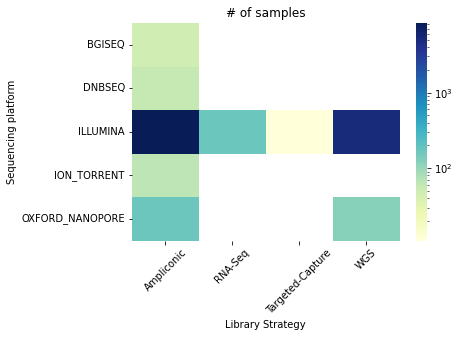
\includegraphics[width=0.7\textwidth]{figures/methods/datasets-heatmap.png}
                \captionof{figure}{Number of samples available for each sequencing platform and library preparation strategy for SARS-CoV-2 in wastewater according to ENA archive as of May 2022. BGISEQ, DNBSEQ, ILLUMINA, ION\_TORRENT, and OXFORD\_NANOPORE refer to corresponding sequencing technologies. Ampliconic library strategy refers to library preparation based on amplicons, while RNA-Seq, Targeted-Capture, and \acrshort{wgs} refer to types of metatranscriptomic-based library preparation strategy.}
                \label{fig:methods:data-heatmap}
            \end{figure}
       
        \subsubsection{Evaluation of the existing Galaxy workflows} \label{sec:methods:existing}
        Galaxy was used as a workflow manager for this thesis. The Galaxy facilitates open and accessible platforms that can ensure data analysis transparency and reproducibility. There are three global Galaxy instances where the workflow can be accessed immediately and for free. Thousands of users can run hundreds of thousands of analyses per month on each system. Using the service, the user will have access to as much computation as they need (with a limit on the number of simultaneous analyses) and 250GB of disk space, which can be increased based on usage. 

        Moreover, Galaxy provides infrastructure that already contains loads of existing tools, and tools can be added to Galaxy with the help of Planemo \cite{planemo}. It serves as a decent basis for workflow development. Additionally, Galaxy provides automated bots \cite{bots2022} for genome data surveillance which opens the opportunity to be used for SARS-CoV-2 wastewater surveillance workflows in order to analyze data regularly.
        
        The four existing workflows are taken as a basis for this thesis. Diagrams that show these workflows step by step are shown in \cref{fig:methods:artic-wf} and \cref{fig:methods:wgs-wf} for the one taken as basis in this thesis, and in \cref{fig:further:ont-wf} and \cref{fig:further:illumina-wf} in \cref{sec:appendix:figures:wfs} that were not taken as basis in this thesis. They show trustworthy results on clinical SARS-CoV-2 data and are expected to perform well on wastewater data. 
        
        Depending on available data and the prevalence of Illumina sequenced data, two out of four Galaxy existing workflows are improved: Illumina-ampliconic oriented (\cref{fig:methods:artic-wf}) and Illumina-metatranscriptomics oriented (\cref{fig:methods:wgs-wf}). 
        \begin{landscape}
        \centering\vspace*{\fill}
        \begin{figure}[ht!]
            \centering
            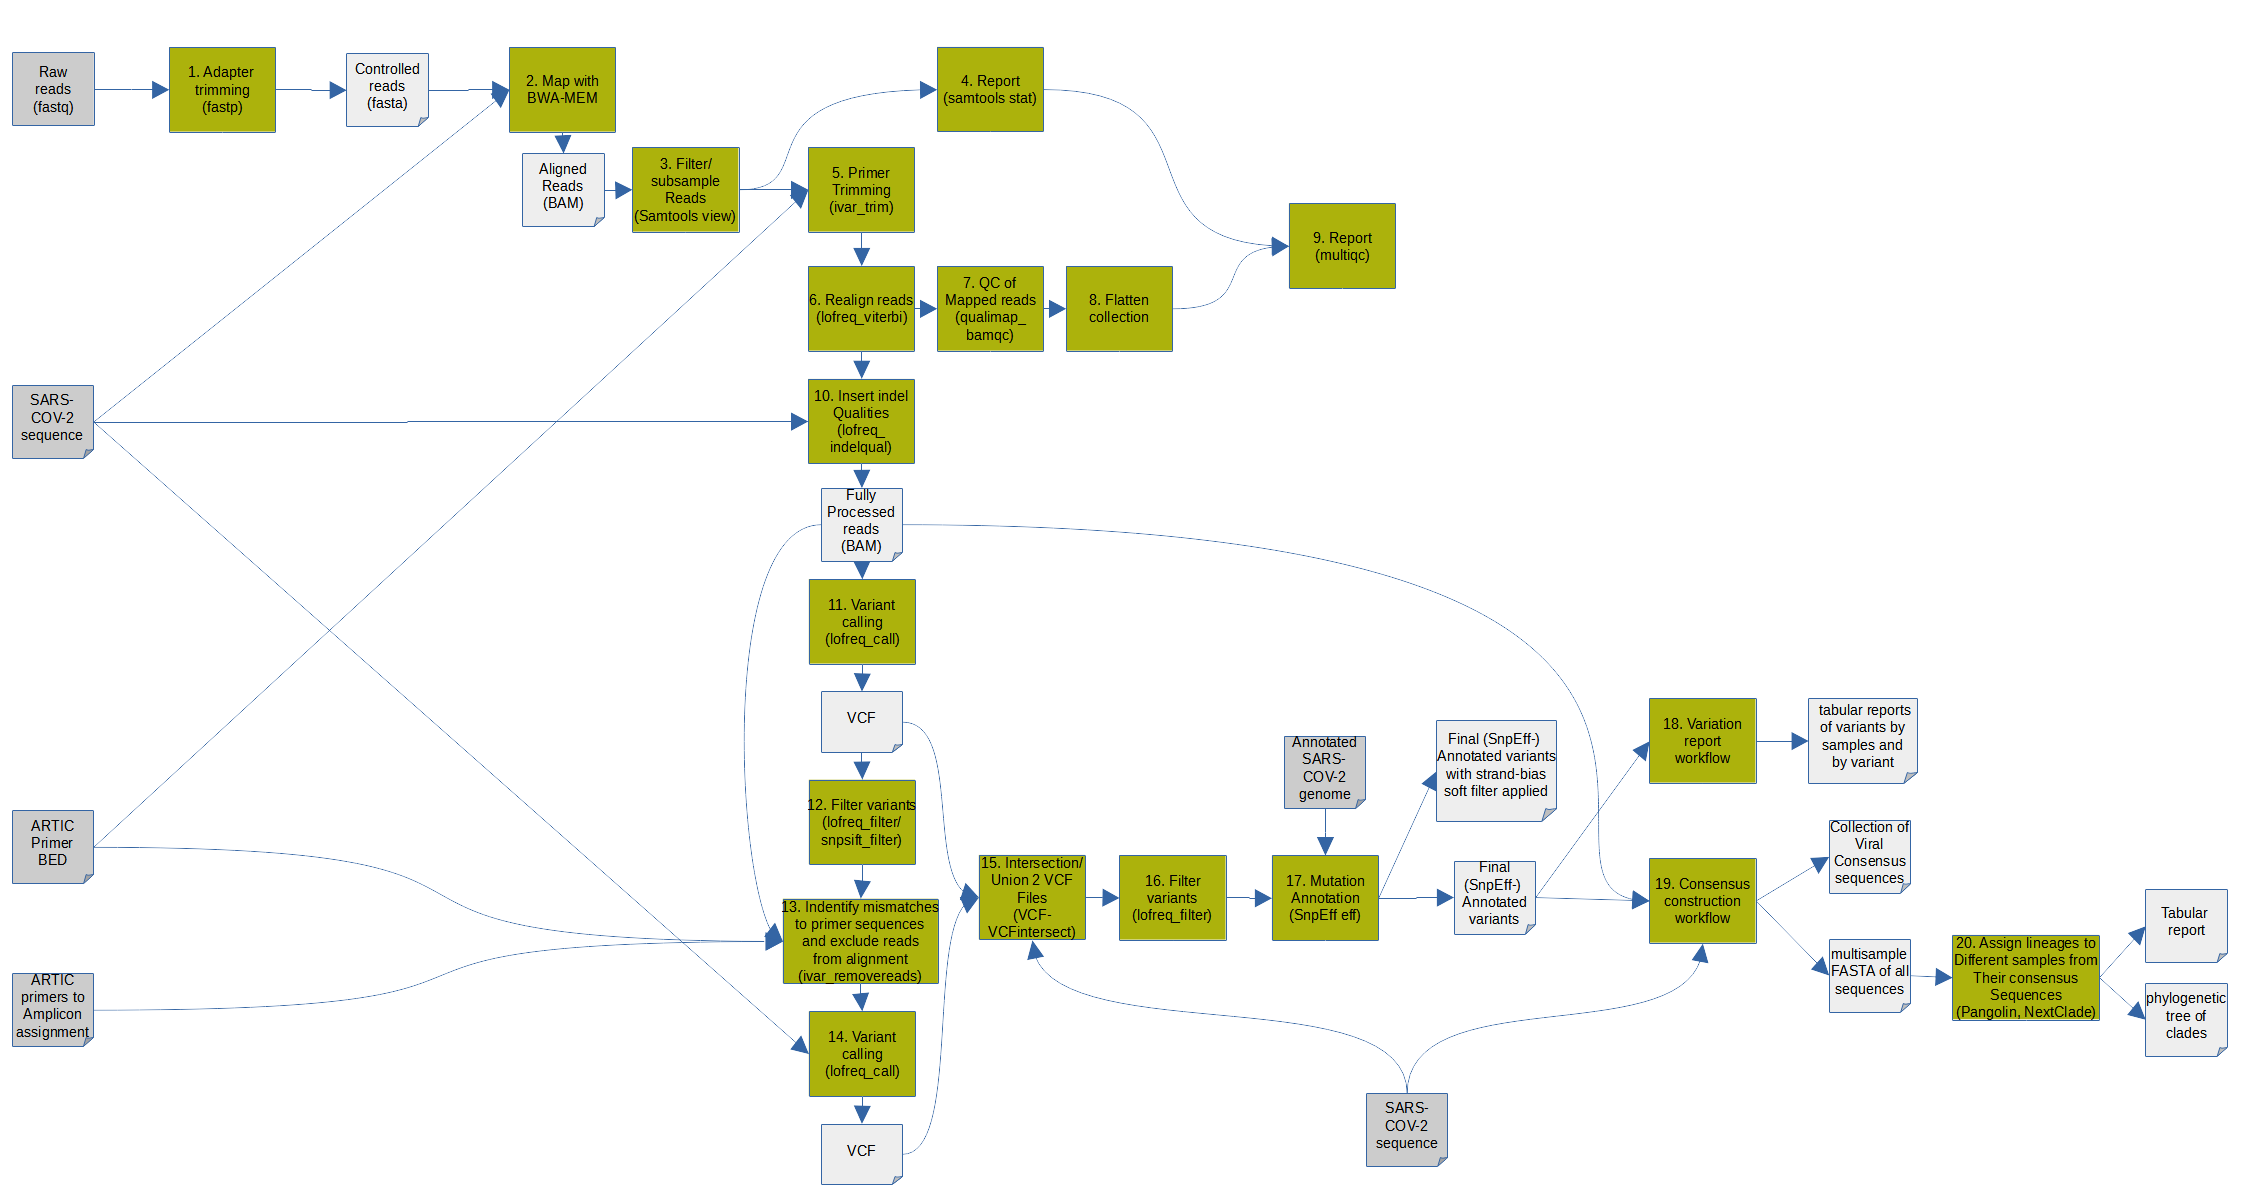
\includegraphics[width=1.4\textwidth]{figures/methods/artic-wf-before.png}
            \captionof{figure}{One of four existing Galaxy workflow for SARS-CoV-2 clinical data surveillance for paired-end reads data extracted with ampliconic-based technique and sequenced with Illumina sequencing approach.}
            \label{fig:methods:artic-wf}
        \end{figure}
        \begin{figure}[ht!]
            \centering
            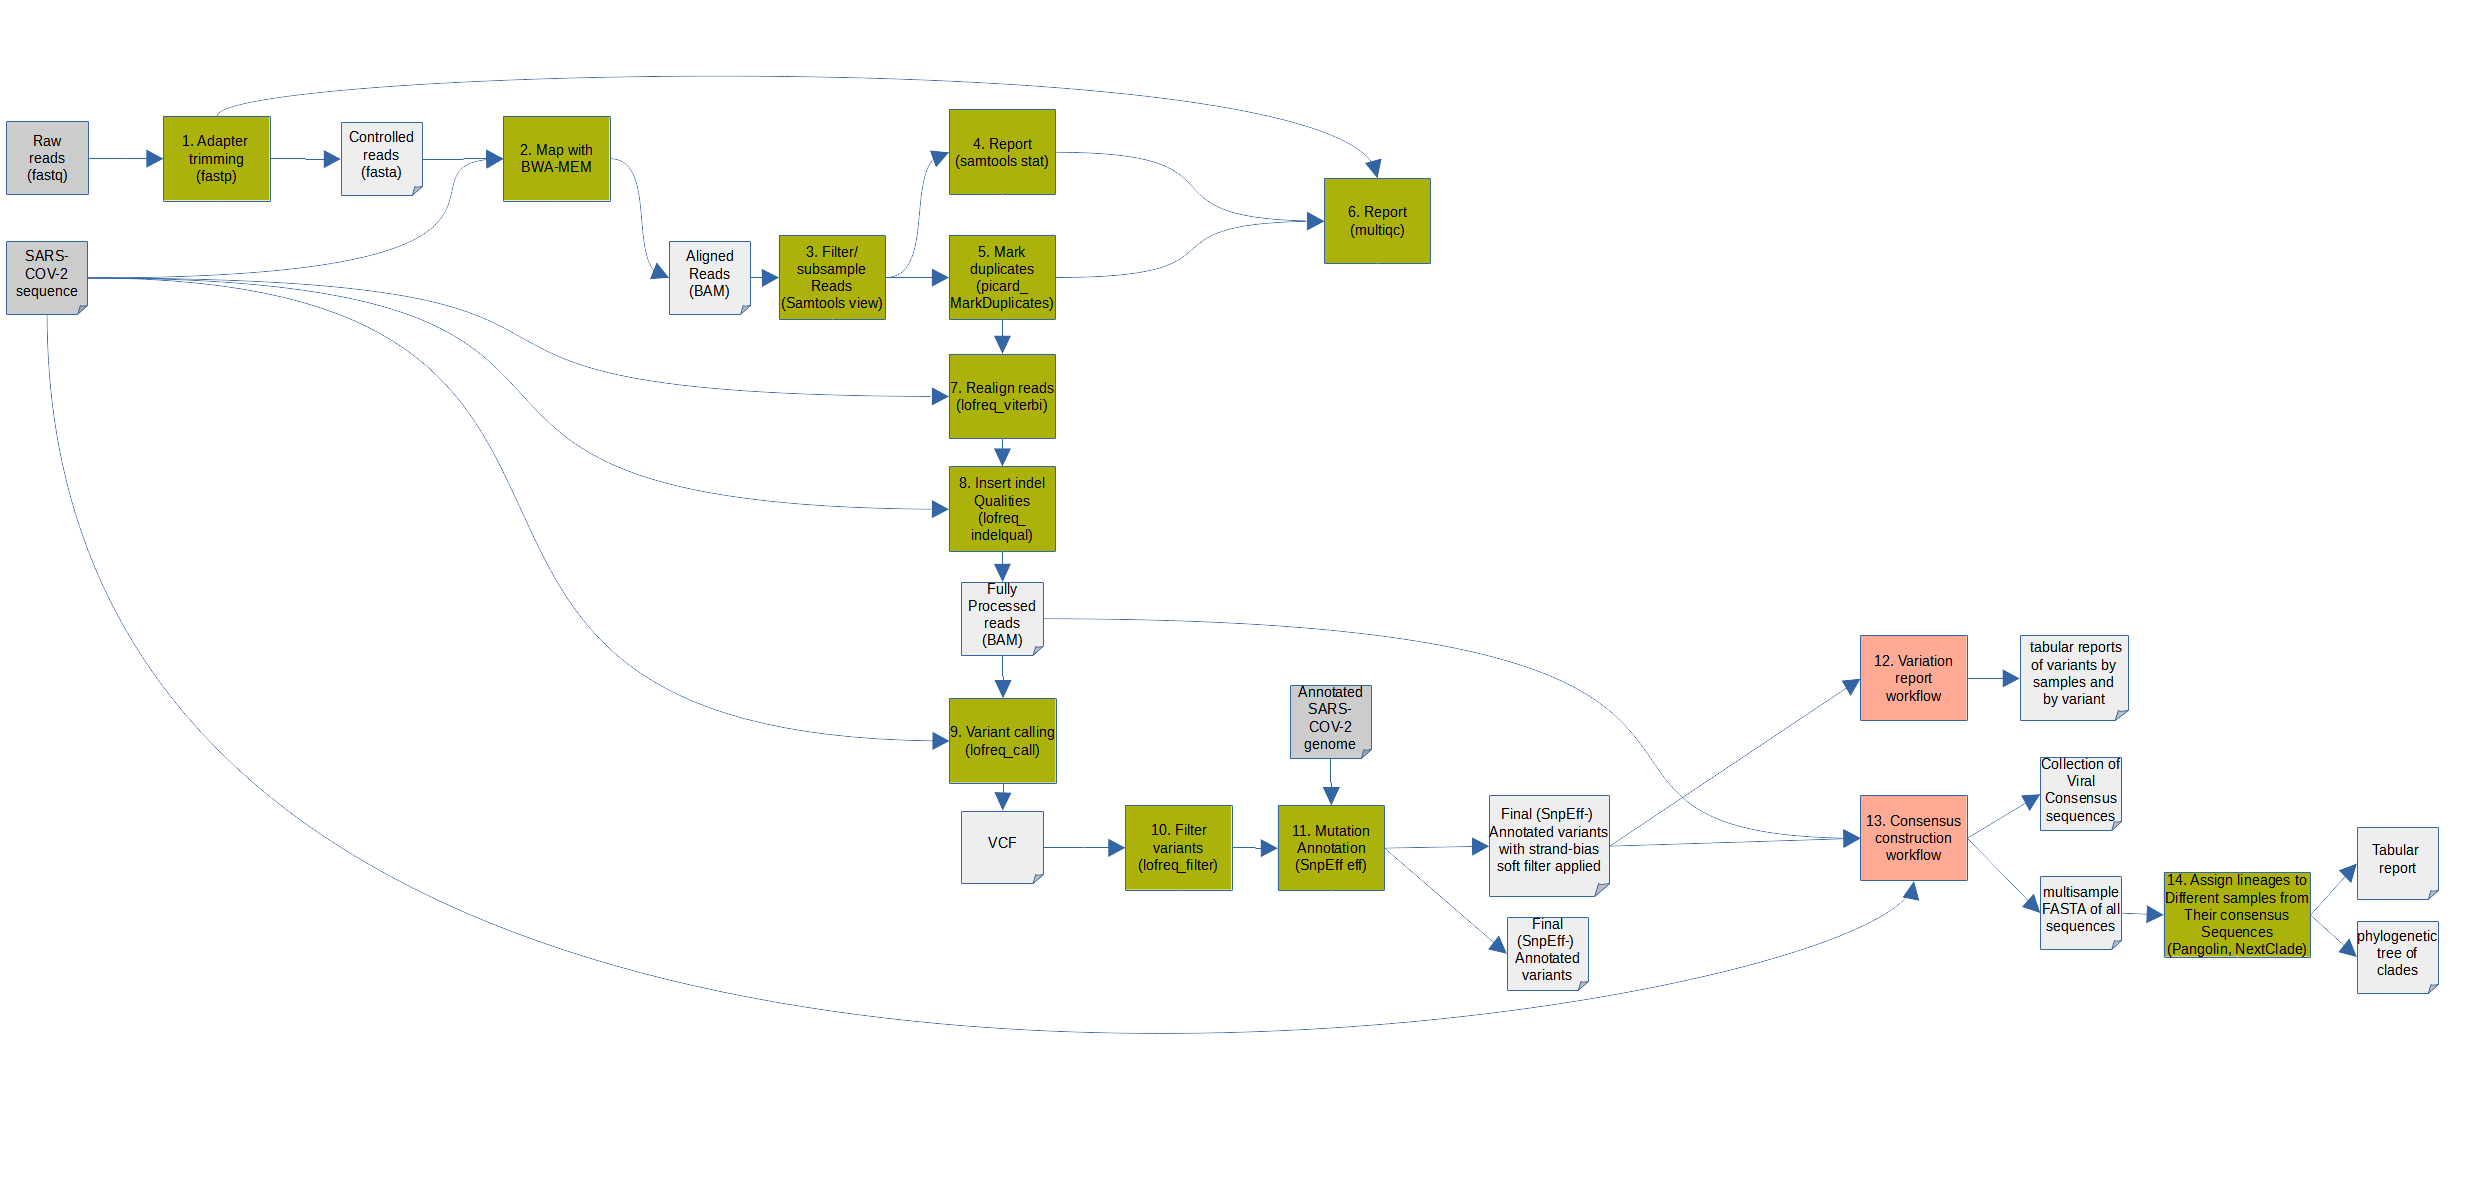
\includegraphics[width=1.4\textwidth]{figures/methods/metatranscriptomics-wf-before.png}
            \captionof{figure}{One of four existing Galaxy workflow for SARS-CoV-2 clinical data surveillance for paired-end reads data extracted with ampliconic-based technique and sequenced with Illumina sequencing approach.}
            \label{fig:methods:wgs-wf}
        \end{figure}
        \vfill
        \end{landscape}
        
        One of the main influences on the decision to take these workflows as a basis for the work in this thesis is preprocessing steps. Preprocessing steps from these workflows were used: i) quality control, ii) adapter trimming, iii) mapping to reference sequence, iv) primer trimming (for the one ampliconic-based where primers were used), v) steps that remove duplicate reads and realign them afterward with reference sequence to prepare data for vi) variant calling. In other words, the sub-workflow for preprocessing data until receiving the VCF file is taken to be: i) improved and ii) extended with the aim of delineating SARS-CoV-2 variants in wastewater samples.Tools differ for different types of datasets and depend on the library preparation approach and sequencing technique as well as on the types of reads obtained (paired-end or single-end). 
        
        In the following \cref{sec:methods:changes}, changes applied to existing Galaxy workflows will be shown, starting with expected input in \autoref{sec:methods:changes:input}, expected output in \autoref{sec:methods:changes:output}, followed by \autoref{sec:methods:changes:improvement} and \autoref{sec:methods:changes:wrappers} where new steps added will be described. Finally, \autoref{sec:methods:changes:step-by-step} will give a picture of workflows improved and repurposed for wastewater surveillance in accordance with the purpose of this thesis. 

        \subsubsection{Changes} \label{sec:methods:changes}
            \paragraph{Input data} \label{sec:methods:changes:input}
            Expected input for both ampliconic-based and metatranscriptomic-based workflows consists of i) a collection of paired-end reads samples of the considered dataset in \acrshort{fasta}/\acrshort{fastq} format; ii) \acrshort{fasta} file of reference SARS-CoV-2 sequence. Additionally, both workflows recommend providing, optionally, though: iii) UShER bar-codes file for lineage assignment used by Freyja; iv) descriptions of variants of concern in \acrshort{json} format used by COJAC. Inputs 3 and 4 are provided by a workflow as well. However, they can be outdated because the updates for both tools happen with a delay. It can happen in case of new variant appearance that up-to-date variants description files are required; hence, the opportunity of submitting them by hand directly to workflow is given.
    
            Moreover, for the workflow that is supposed to work with ampliconic-based datasets extracted using ARTIC protocol, the following input data is necessary: v) \acrshort{bed} file with ARTIC primers description; vi) description file of ARTIC primers to amplicon assignments that is ued by iVar trim and iVar removereads for assigning primers to amplicons. 

            \paragraph{Output data} \label{sec:methods:changes:output}
            In both (ampliconic-based and metatranscriptomic-based) workflows, two distinct branches are developed. The first branch focused on using Freyja tool and its outputs, while the second branch produces results based on COJAC tool usage. The user is provided to use only one of these branches as well as both of them simultaneously. Therefore, depending on the branch run in this workflow, different outputs will be obtained.
            
            The first option is based on Freyja tool for the delineation of SARS-CoV-2. Due to Freyja's use of the UShER phylogenetic tree, the output of the workflow is high-level rough reports, the proportions of specific lineages (e.g. Omicron, Delta, etc.), and their co-occurrences. Reports in this branch can be made in PDF and HTML interactive formats. Additionally, if the metadata file describing samples metadata (date of collection, viral load, etc.) is provided by a user, various plots show the dynamics of SARS-CoV-2 over time.
            
            The second branch, in turn, is based on COJAC tool for delineation. These tools provide more detailed information about variants of concern. It is possible to describe new variants in COJAC that can turn into \acrshort{vocs}. This feature makes it possible to use this tool and the COJAC-based workflow to connect with CoV-Spectrum. Even though the script for upload to CoV-Spectrum is not automated yet, it can be applied separately based on tabular output from COJAC. 

            \paragraph{Improvement of preprocessing subworkflows} \label{sec:methods:changes:improvement}
            The initial phase of workflows development in this thesis is to take subworkflows from existing workflows responsible for data preprocessing and improve them, taking into account the goal of wastewater surveillance. 

            One of the improvements made in workflows is the addition of a decontamination step. There were several reasons why a decontamination step was added to the workflow. The first and foremost reason is to eliminate any potential concerns about the anonymity of the host of the virus. Considering that SARS-CoV-2's hosts are predominantly humans and in this master thesis, I am working with wastewater which by default contains the human genome, that seemed to be a good idea to decontaminate samples from the human genome in the beginning. Additionally, this step is added to improve the runtime and accuracy of mapping from the sequence of a virus to a reference virus sequence. 
            
            Including decontamination in workflows relies on the fact that human contamination is inevitable in wastewater samples. ReadItAndKeep tool \cite{hunt2022} was added after adapter trimming (with Fastp tool) for both workflows to only keep reads matching the SARS-CoV-2 genome so that host reads could be removed from sequencing data for SARS-CoV-2. 
            
            Another step added to both workflows is a taxonomic analysis of reads that are unmapped to reference SARS-CoV-2.  I added two tools, Kraken 2 \cite{wood2014,wood2019,lu2020} and Visualization with Krona chart \cite{ondov2011,cuccuru2014}. 
            
            The tool Kraken 2 is a taxonomic sequence classifier that classifies reads according to their taxonomic labels. In order to accomplish this, it examines the k-mers within a read and queries a database with them. A taxonomic tree of all genomes that contain a given k-mer contains a mapping from Kraken's genomic library to its \acrfull{lca}. To create a taxonomic label for a read, the \acrshort{lca} taxa corresponding to its k-mers are analyzed. Labels can refer to any of the taxonomic nodes. In workflows, the viral genomes database was applied.
            
            The other tool, Krona chart, is an intuitive visualization tool that helps visualize relative abundances and confidences in multiple metagenomic classifications. Radial, space-filling displays are combined with parametric coloring and interactive zooming in polar coordinates in Krona. Using HTML5 and JavaScript, the charts can be interactively explored by any Web browser \cite{ondov2011}.
            
            It is possible to use these tools to learn about other species of bacteria that can be found in wastewater samples in addition to SARS-CoV-2. A taxonomical analysis, as well, opens the possibility of detecting newly emerged variants of SARS-CoV-2 because otherwise, they would not be able to match reference sequences and, therefore, will not be noticed. By taking this additional step, we close not only the interest in other species that wastewater samples contain and can be useful outside of SARS-CoV-2 topic but also contribute to the possibility of catching new variants of SARS-CoV-2. 
            
            One other step that should be mentioned is computing sequence depths with Samtools depth \cite{li2009}. It was added into both workflows after mapping to the reference step because the information about sequencing depths is required as input for the demixing command of Freyja tool.
            
            \paragraph{Tool integration} \label{sec:methods:changes:wrappers}
            Apart from the improvement of the existing preprocessing sub-workflow, new steps were added with the intention to reaching the goal of this thesis: to identify SARS-CoV-2 lineages in wastewater samples. In this regard, I have added delineating steps to both branches of the workflow based on Freyja and COJAC tools. These tools were chosen as individual tools that can be plugged into Galaxy workflow and represent different types of SARS-CoV-2 lineages abundances analysis and outputs that can be benchmarked afterward with each other as well as with outputs from the outside non-Galaxy standalone workflow for evaluation.

            To facilitate this master thesis, I developed Galaxy wrappers for tools that did not have one.  For that, I used Planemo \cite{planemo}, a command-line application for creating Galaxy tools, workflows, and training materials. Planemo is also used to deploy tools and workflows (tools to Galaxy ToolShed; workflows to Intergalactic Workflow Commission) as well as execute Galaxy-based analyses by command line if one prefers that interface to Galaxy's graphical interface.
            
            In designing both tools, detailed consideration was given to the user interfaces. A wrapper was designed not only to accommodate the needs of this master thesis research but also to be able to be used by researchers who are interested in using both tools independently on any Galaxy instance (e.g. \url{https://usegalaxy.eu/}, \url{https://usegalaxy.com/}, \url{https://usegalaxy.org.au/}, etc.) and also included in the specific workflow. While designing tool wrappers, enough effort was put in, in order to make the interface convenient as well as functional.
            
            For example, features like samples name autodetection and the option to provide samples names by the user, or the option to use variant descriptions of SARS-CoV-2 variants of concern cached in Galaxy as well as the option to provide the user's preferred list of variant descriptions were included. Another example is the ability to combine different types of output plots for Freyja. Additionally, for COJAC, the possibility of receiving various output tables (e.g. line-oriented, column-oriented, or multilevel-oriented) was provided. 
            
            Overall, for Freyja tool, there were four wrappers created: i) Freyja: Call variants and get sequencing depth information (although, it was not needed for this thesis because Galaxy workflows are elaborated to call variants in a more precise way); ii) Freyja: Bootstrapping method, which was not used in this thesis either but was designed anyway for the perspective usage by interested users; iii) Freyja: Demix lineage abundances; iv) Freyja: Aggregate and visualize demixed results. Throughout this thesis, the last two tools were applied to both workflows.
            
            Withal, for COJAC tools, there were three wrappers designed: i) Cojac: mutbamscan scan an alignment file for mutation co-occurrences (the output is generated in \acrshort{json}, \acrshort{yaml}, and/or \acrshort{csv} table format); ii) Cojac: tabmut export cooccurrence mutations as a table (that interprets Cojac mutbamscan into nicer and readable tabular format); iii) Cojac: pubmut render a \acrshort{json} or \acrshort{yaml} file to a pretty table (that produces output in \acrshort{csv} and/or \acrshort{html} format which is pretty enough to be included in publications). Cojac: pubmut was added to Galaxy only for the case of potential interest in it outside workflows and was not directly used in the workflows developed to achieve the thesis's goal. Cojac: mutbamscan and Cojac: tabmut, in their turn, were used in the workflow corresponding to data obtained with the ampliconic library preparation method. Although COJAC can work with ampliconic data, it was not created to work with metatranscriptomic data. 
            
            Once wrappers are ready and tested, I contributed to galaxyproject/tools-iuc (available in the fork \url{https://github.com/PlushZ/tools-iuc}) to make Freyja and COJAC available to Galaxy. The tools were also added to usegalaxy.eu. 
            
            \paragraph{Workflows step by step} \label{sec:methods:changes:step-by-step}
            The final workflows developed in this master thesis are depicted in \cref{fig:methods:artic-wf-after} and \cref{fig:methods:wgs-wf-after} for Illumina ampliconic paired-end SARS-CoV-2 wastewater surveillance and for Illumina metatranscriptomic paired-end SARS-CoV-2 wastewater surveillance, respectively. In green, steps kept from existing Galaxy workflows for clinical SARS-CoV-2 data surveillance are depicted. Newly added steps for the target of this master thesis are indicated in orange. On the diagram, there is also a step called CoV-Spectrum colored pink. So far, this step is not automated and can be done only manually. Nonetheless, future improvements outside of this thesis could automate this step.
            \begin{landscape}
            \centering\vspace*{\fill}
            \begin{figure}[ht!]
                \centering
                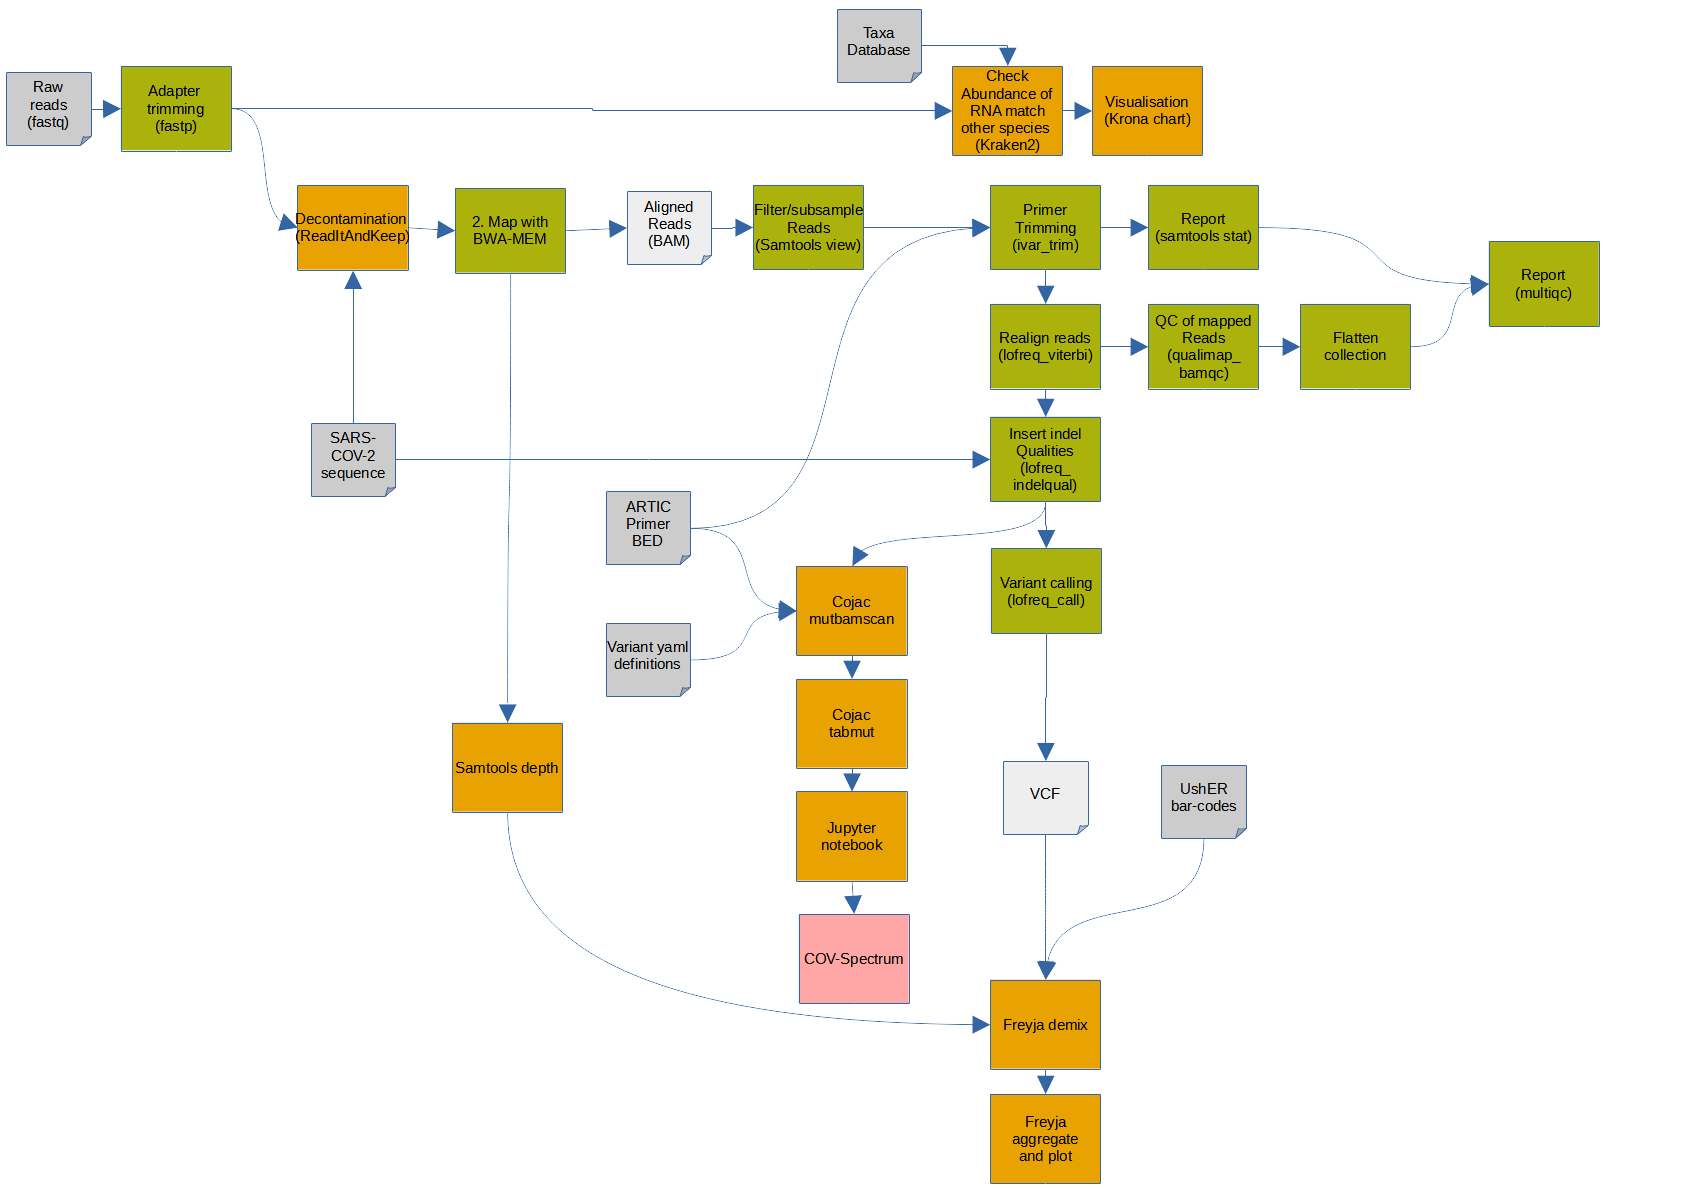
\includegraphics[width=1.2\textwidth]{figures/methods/artic-wf-after.png}
                \captionof{figure}{Improved and repurposed to SARS-CoV-2 wastewater surveillance Galaxy workflow for paired-end data extracted with ampliconic-based technique and sequenced with Illumina sequencing approach.}
                \label{fig:methods:artic-wf-after}
            \end{figure}
            \begin{figure}[ht!]
                \centering
                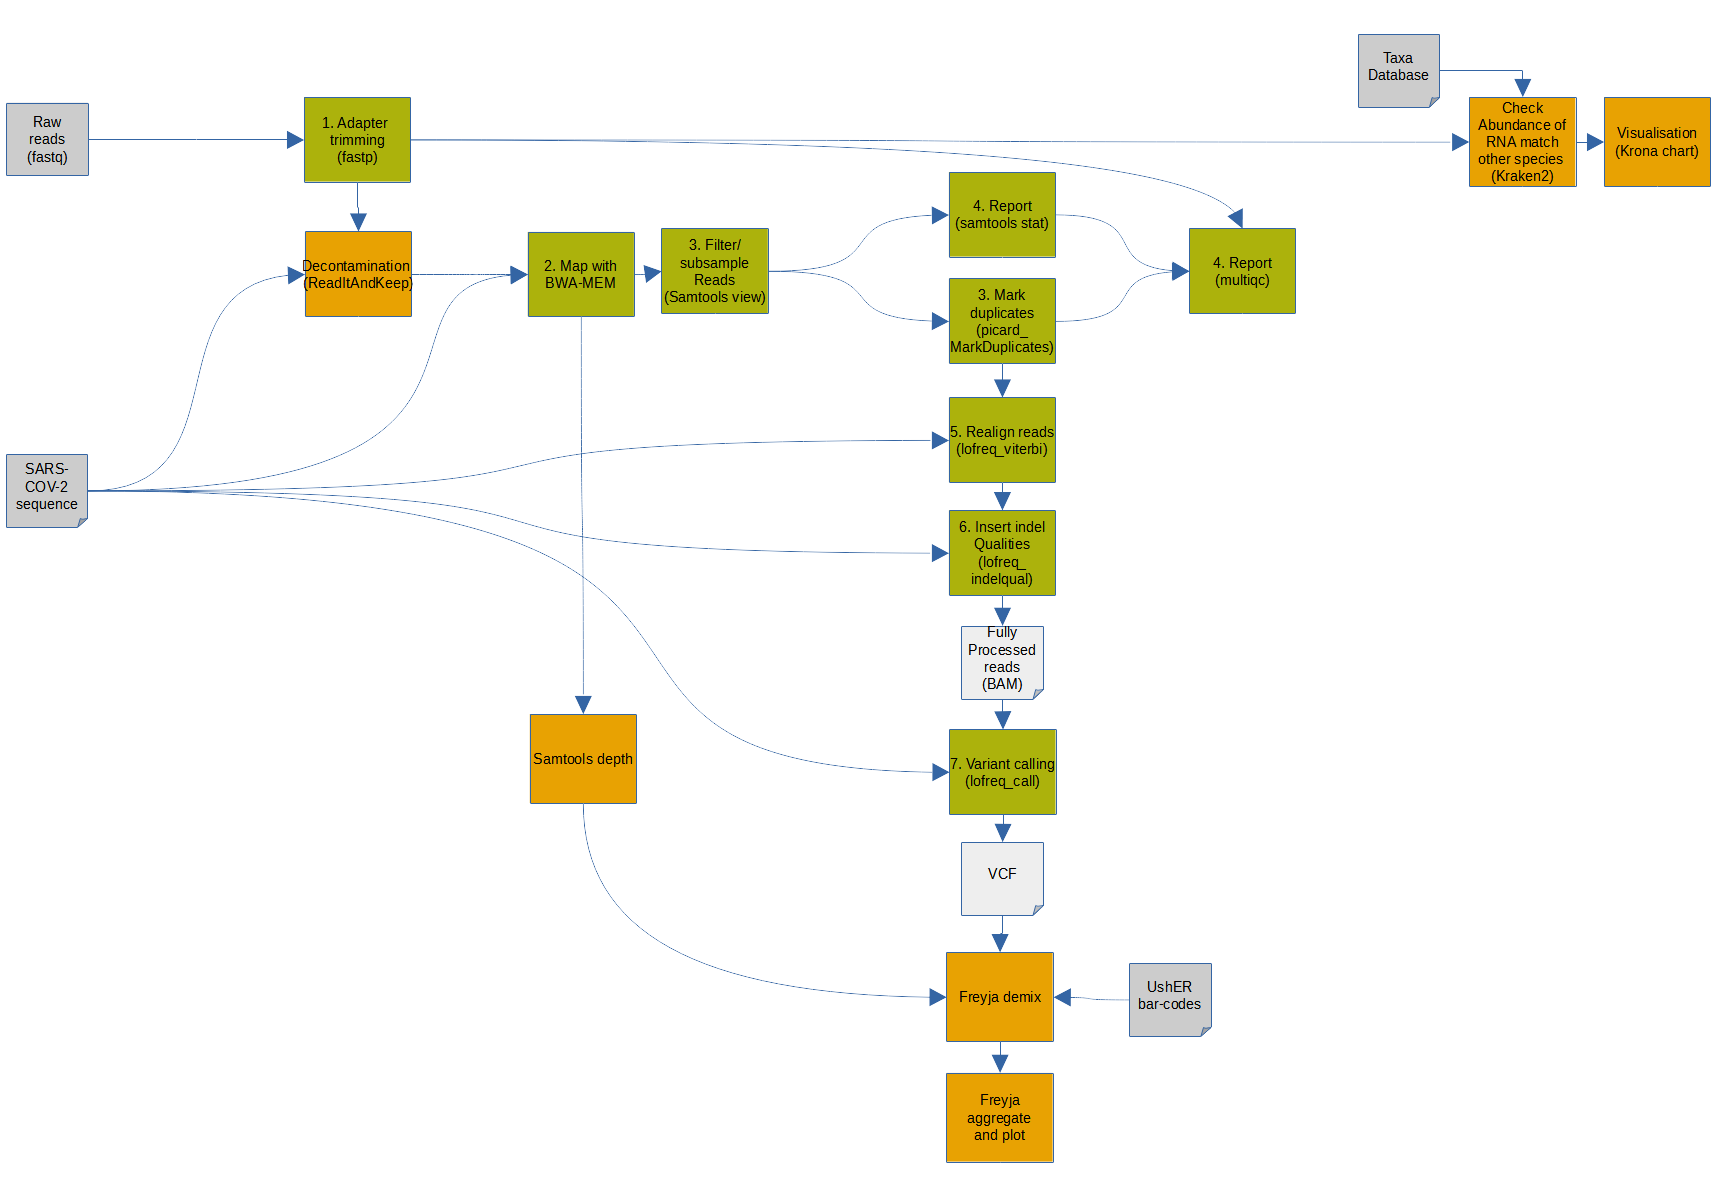
\includegraphics[width=1.3\textwidth]{figures/methods/metatranscriptomic-wf-after.png}
                \captionof{figure}{Improved and repurposed to SARS-CoV-2 wastewater surveillance Galaxy workflow for paired-end data extracted with metatranscriptomics-based technique and sequenced with Illumina sequencing approach.}
                \label{fig:methods:wgs-wf-after}
            \end{figure}
            \vfill
            \end{landscape}
        
    \subsection{Workflow evaluation} \label{sec:methods:evaluation}
    To assess the quality of developed workflows, I used a synthetically generated mock dataset and compared results obtained by the developed Galaxy workflow with expected ground truth results from the information about generated mock dataset. In addition, results from Galaxy workflow were benchmarked with the results from another solution, namely Lineagespot. Afterward, I launched both workflows on four real-world datasets mentioned in \cref{sec:methods:needs}.
        
        \subsubsection{Evaluation on mock data} \label{sec:methods:evaluation:mock}
            \paragraph{Generated mock datasets}
            Generated synthetic dataset was created by a working group and is uploaded in \href{https://github.com/suskraem/ww_benchmark}{Github repository} available under an open source license \cite{benchmarksamples}. Synthetic datasets were created by obtaining genomes from the Pango designation list. While generating synthetic mock data, the focus was on 3 real variants (BA.1, BA.2, Delta), one synthetic 'background' (BG) variant to mimic the effect of an unknown variant, as well as recombinant genomes (Omicron-Delta) \cite{simonloriere2011,variants}. Synthetic 'amplicons' were created using ARTIC v4.1 primers. Synthetic reads were created using error models based on 150 or 250bp NovaSeq reads. There were created samples belonging to groups of different classes such as: i) Single lineage, Two lineages, Three lineages; ii) High coverage, Low coverage; iii) Long reads, Short reads. In \cref{tab:methods:mock}, classes used to generate synthetic mock dataset are listed.
            
            \begin{table}[H]
            \centering
            \small
            \begin{tblr}{l|[dashed]llll}
            \textbf{Number}             & \textbf{Lineages}             & \textbf{Coverage}                   & \textbf{Read}          & \textbf{Number}  \\ 
            \textbf{of lineages}         &                              &                                     & \textbf{length, bp}           & \textbf{of samples} \\ \hline
            Single lineage          & BA.1                              & high                          & 150                               & 2 \\
                                    &                                   & low                           & 150                               & 2 \\
                                    &                                   &                               & 250                               & 2\\ \cline[dashed]{2-5}
                                    &  \textbf{BA.1 Total}              &                               &                                   & \textbf{8} \\\cline[dashed]{2-5}
                                    & BA.2                              & high                          & 150                               & 1 \\
                                    &                                   &                               & 250                               & 1 \\
                                    &                                   & low                           & 150                               & 1 \\
                                    &                                   &                               & 250                               & 1\\ \cline[dashed]{2-5}
                                    &  \textbf{BA.2 Total}              &                               &                                   & \textbf{4} \\\cline[dashed]{2-5}
                                    & Delta                              & high                          & 150                               & 1 \\
                                    &                                   &                               & 250                               & 1 \\
                                    &                                   & low                           & 150                               & 1 \\
                                    &                                   &                               & 250                               & 1\\ \cline[dashed]{2-5}
                                    &  \textbf{Delta Total}              &                               &                                   & \textbf{4} \\\cline[dashed]{2-5}
                                    &                                   &                               & 250                               & 1 \\
                                    &                                   &                               & 250                               & 1\\ \cline[dashed]{2-5}
                                    &  \textbf{Recombinant Total}       &                               &                                   & \textbf{2} \\\cline[dashed]{2-5}
                                    & Synthetic lineage                 & high                          & 150                               & 1 \\
                                    &                                   &                               & 250                               & 1 \\
                                    &                                   & low                           & 150                               & 1 \\
                                    &                                   &                               & 250                               & 1\\ \cline[dashed]{2-5}
                                    &  \textbf{Synthetic Total}         &                               &                                   & \textbf{4} \\\hline[dashed]
            \textbf{Single lineage Total} &                                  &                               &                                   & \textbf{22} \\ \hline
            Two                     & BA.1:BA.2                         & high                          & 250                               & 3 \\
             lineages               &                                   & low                           & 250                               & 3 \\\cline[dashed]{2-5}
                                    &  \textbf{BA.1:BA.2  Total}       &                               &                                   & \textbf{6} \\\cline[dashed]{2-5}
                                    & BA.1:Delta                         & high                          & 150                               & 7 \\
                                    &                                   &                               & 250                               & 14 \\
                                    &                                   & low                           & 150                               & 7 \\
                                    &                                   &                               & 250                               & 14\\ \cline[dashed]{2-5}
                                    &  \textbf{BA.1:Delta Total}        &                               &                                   & \textbf{42} \\\hline[dashed]
            \textbf{Two lineages}   &                                  &                               &                                   & \textbf{48} \\
            \textbf{Total}          &                                  &                               &                                   & \\\hline
             Two lineages           & BA.1:Delta:Synth                  & high                          & 250                               & 7 \\
            + Synthetic            &                                   & low                           & 250                               & 7 \\
             lineage               &                                   &                               &                                & \\ \hline[dashed]
                                    &  \textbf{BA.1:Delta:Synth Total}  &                               &                                   & \textbf{14} \\ \hline
            \end{tblr}
            \end{table}
            \begin{table}
            \begin{tblr}{l|[dashed]llll}
            \textbf{Number}             & \textbf{Lineages}             & \textbf{Coverage}                   & \textbf{Read}          & \textbf{Number}  \\ 
            \textbf{of lineages}         &                              &                                     & \textbf{length, bp}           & \textbf{of samples} \\ \hline
               Three                 &      BA.1:BA.2:Delta             &      high                         & 250                       & 4 \\
                lineages            &                                   &    low                           & 250                              & 4\\ \hline[dashed]
                                    &  \textbf{BA.1:BA.2:Delta Total}  &                               &                                   & \textbf{8} \\ \hline
                Three  lineages     &      BA.1:BA.2:Delta:Synth        &      high                     & 250                               & 4 \\
                + Synthetic          &                                   &    low                           & 250                           & 4\\ \hline[dashed]
                lineage              &  \textbf{BA.1:BA.2:Delta:Synth Total}  &                          &                                   & \textbf{8} \\ \hline
                \textbf{Total}      &                                    &                               &                                   & \textbf{100} \\ \hline

            \end{tblr}
                \caption{Overall numbers of samples, sorted by various groups of samples from the generated synthetically mock dataset. The table was created using a PivotTable in Google Sheets. Metadata about samples in the mock dataset was uploaded to Google Sheets, then, Pivot table was generated to analyze numerical data. First, data was sorted by Number of lineages, followed by sorting by exact Lineages combination, Coverage, and Read length. Next, the sum of samples for every class was calculated.} \label{tab:methods:mock}
            \end{table}

            Overall, the mock dataset contains 100 samples. More specifically, it contains 22 samples with single lineage, 42 with two distant lineages (BA.1 and Delta), 6 samples with two close lineages (BA.1 and BA.2), 14 samples with 2 known and one unknown lineage (synthetically generated), 8 samples with known lineages, and 8 samples with 3 known and one unknown lineages. In terms of coverage, the mock dataset contains 50 samples of low coverage and 50 samples of low coverage. In terms of read length, there are 24 samples of long reads (250 base pairs) and 76 samples of short reads (150 base pairs).
            
            In order to evaluate and draw conclusions about the performance and efficiency of developed workflows, the workflow for ampliconic-based data was run on a mock dataset along both branches: Freyja-based and COJAC-based. Aside from Galaxy, Lineagespot standalone workflow was launched in parallel on the same mock dataset for benchmarking all three methods' results.
            
            \paragraph{Comparison of proposed workflows} 
            To compare two branches of the proposed Galaxy workflow (with Freyja and with COJAC) and evaluate Galaxy workflow results, I examined them with the known expected results. Knowing the ground truth results allows me to draw conclusions about the performance of developed workflows and their accuracy. 
            
            For further evaluation, resulting data were divided according to the principle of belonging to a particular expected group. The groups of greatest interest were: Single lineage expected to be found in the sample and Two lineages.
            
            Even though both Freyja and COJAC methods found extra lineages that were not expected, I focused on their capability to detect expected lineages (Delta, BA.1, and BA.2) in abundance proportion closer to the expected proportion.

            
                \subparagraph{Preprocessing data} 
                Data obtained by Freyja and COJAC were preprocessed to make them comparable. Data from Freyja were obtained in \acrshort{tsv} (tabular) format (as shown for sample1 example in \cref{list:methods:freyja-s1}). To distinguish variants Delta, BA.1, and BA.2, which are focused on the mock dataset, a simple Python script (provided in \cref{list:methods:freyja-vocs-abundances}) was used considering that Delta lineage as B.1.617.2 and its sublineages starting with AY according to Pango designation \cite{otoole2021,covlineages}. In COJAC, in its turn, proportions of lineage abundances are computed for every amplicon, and for every lineage, a median of abundance proportion among different amplicons was computed.
                
                \begin{lstlisting}[language=xml, caption=Freyja output for sample 1 from mock dataset, label=list:methods:freyja-s1]
 Sample name	summarized	lineages	abundances	resid	coverage
 sample1 	[('Omicron', 0.6999889999983451), ('Delta', 0.22408099987442534), ('Other', 0.07552100018490182)]	BA.1.18 AY.4 BA.1.19 BA.1.1.13 BA.1.15.1 AY.38 BA.1.9 BA.1.16 B B.1.617.2 B.1.1.529 XS	0.23943700 0.11764700 0.11363600 0.10000000 0.09667000 0.06944400 0.06686400 0.06474800 0.06122400 0.03699000 0.01863400 0.01429700	7.611495978	99.95971667
                \end{lstlisting}
                
                To work with resulting output data from both branches of Galaxy workflow, they were stored in google sheets. Python pandas data analysis tool \cite{pandas2022} was used to access data and create dataframes from the data obtained. Dataframes were then used for downstream analysis.

                \subparagraph{Comparison}
                Parallel coordinates plot was created for detected proportions of different lineages using Python and Plotly graphing library \cite{plotly}. Three plots were generated for Delta, BA.1, and BA.2 lineages. First, I plotted all samples in one plot without their division into groups. All 100 samples were included in the first three plots in order to get an overall imagination of lineage proportion distribution among samples and their comparison to expected proportion values. Plots are available in \autoref{sec:appendix:figures:parallel-all} of \cref{sec:appendix}. The first axis is the Expected proportion, the second is the result obtained by COJAC, and finally, the third is Freyja’s proportion of the considered lineage of SARS-CoV-2. Additionally, I generated one plot per considered lineage (Delta, BA.1, or BA.2) and per group of samples (Single lineage expected, Two lineages expected). Overall, 6 plots were created. 

                To zoom up, the focus on one sample was done. Hence, there were generated for every sample: parallel coordinates plot and bar plot using Seaborn Python library, and line plot using Matplotlib (to look at absolute values of lineage proportion against scaled values in parallel coordinates). The comparison with expected lineage proportions was included in these plots.
                
                To compare Freyja and COJAC branches of workflow and to assess results with expected ones, I took a look at the distribution of Delta lineage proportion in the sample (obtained by Freyja, COJAC, and expected proportion) across all samples. The same comparison was made for BA.1 and BA.2 lineages.
                
                Other angle to look at results is to see a distribution of proportion of all three considered lineages across samples for both Freyja and COJAC. Thus, a distribution plot using Python and Seaborn library was generated. To be said, the similar distribution plot of proportion of all three considered lineages across samples for Lineagespot was generated analogously to plots for Freyja and COJAC.

                
            \paragraph{Comparison with lineagespot} \label{sec:methods:evaluation:mock:compare-ls}
            For the comparison of proposed Galaxy workflow results with Lineagespot results, the same synthetic mock dataset was used. Lineneagespot results on the mock dataset were obtained following private communication with F. Psomopoulos \cite{pechlivanis2022}. It was expected that the results of both branches of Galaxy workflow turned out to be different from the results of Lineagespot. That is because different approaches (sub-workflows) are used for the variant calling steps. In the case of Galaxy workflow, LoFreq variant caller is used preceding several steps for primer trimming, realignment, and insertion of indel qualities (using LoFreq\_insertindel). On the other hand, Lineagespot uses duplicates filtering with Picard tool, followed by variant calling with Freebayes tool. For lineage annotation, also different approaches are used. While for Galaxy workflow, Frejya or COJAC are options, Lineagespot pipeline uses its own approach for delineation. Thus, results from Galaxy workflow, whether Freyja-based or COJAC-based, are expected to differ.

            Data obtained from Lineagespot was already preprocessed, proportions of expected lineages were provided as well as assignments to certain lineages. To compare the results of Lineagespot and Galaxy workflows, Freyja-based or COJAC-based, against each other and against expected results, I focused specifically on two groups of samples from the mock dataset: the group where single lineage was expected (22 samples) and the group where two lineages were expected (48 samples). 

            
                \subparagraph{Single lineage group of samples} 
                For a single lineage group of samples, four characteristics were used. I intended to learn in which samples were detected: i) expected lineage; ii) expected+unexpected lineages; iii) unexpected lineage; iv) nothing. For each of these characteristics, bar plots were created separately, as well as a combined barplot that shows the number of samples that satisfy each characteristic. Also, a barplot was generated showing the percentage of samples that belong to each characteristic.

                Further, considering only samples where expected lineage was detected, the distribution of lineage proportion detected by Freyja and COJAC among samples of the Single lineage group was plotted with Python with the help of Seaborn library. Only Freyja and COJAC were compared. I do not consider Lineagespot here because in the results of Lineagespot I do not have a clean proportion distribution between lineages. There is no information about other lineages detected (aside from BA.1, BA.2, Delta), while the sum of proportions of these three is not equal to 1 in Lineagespot.
                
                To better understanding relationships between sets of different methods (Freyja, COJAC, Lineagespot) results, Venn Upset diagram was generated. The goal was to look at intersections between sets of results and which samples were detected correctly (in terms of lineages expected) by which tool and to find similarities in tools performance.

            
                \subparagraph{Two lineages group of samples}
                As for the group of samples where two lineages are expected to be found, I defined 5 characteristics depending on what was detected in samples: i) both expected lineages; ii) only one expected lineage; iii) one expected+unexpected lineages; iv) both expected+unexpected lineages; v) nothing. Similarly to the single lineage group of samples analysis, for each of these characteristics, barplots were created using Python separately as well as a combined barplot that shows the number of samples that satisfy each characteristic. Additionally, there was a barplot created showing the percentage of samples that belong to each characteristic.

                To zoom in, analysis was done for the most interesting sub-group of the group of samples where two lineages are expected to be detected. In this sub-group, there are two types of samples where both expected lineages are detected, and both expected + unexpected lineages are detected. To compare results, it is reasonable to look at the correlation between specific lineages, such as Delta, BA.1, and BA.2, as in this mock dataset, only three known lineages were used. The first option is to look at the ratio between BA.1 and BA.2 lineages. The second option is the relation between BA.1 and Delta lineages. The third is BA.2 and Delta relation. However, the third option does not make sense in this mock dataset because there are no samples in the group of two lineages where these two appear together at the same time.
                
                Therefore, in total, 6 cases were considered: i) BA1 > BA2; ii) BA1 = BA2; iii) BA1 < BA2; iv) BA1 > Delta;  v) BA1 = Delta;  vi) BA1 < Delta. 
                I looked at every case where this relation was expected and compared obtained results from Freyja, COJAC, and Lineagespot regarding the relation between two certain lineages (BA.1/BA.2 relation and BA.1/Delta relation). To visualize results, 6 bar plots were generated and explained in \cref{sec:results}.
                
                To better understand relationships between sets of different methods (Freyja, COJAC, Lineagespot) outputs, Venn Upset diagram was generated. The goal was to look at intersections between sets of results and in which samples both lineages were detected correctly (compared to expected ones) by which tool and to find similarities in tools' performance.
                
                All plots are shown in \cref{sec:results}.

        
        \subsubsection{Evaluation on real-world data} \label{sec:methods:evaluation:real}
        
            \paragraph{Chosen real-world datasets} 
            In order to provide a fairly comprehensive analysis, real-world datasets for experiments in this thesis were selected in such a way that they cover a variety of locations in the world and different time points of collecting samples. In this way, it was expected to obtain data on the evolution of SARS-CoV-2 over time, as well as data on which variants prevailed in which countries at these time points. This variety of datasets considered in this thesis can be in the future regularly analyzed using automatized Galaxy bot like it is currently managed for clinical data. 

            Choice of my thesis fell on the four datasets: i) one dataset from California (PRJNA661613)\cite{critschristoph} where the samples were collected in 2020 at a wastewater interceptor (labeled Berkeley, Berkeley Hills, Oakland, and Marin, according to the municipal areas each serves); ii) a dataset from the UK (PRJEB42191) \cite{hillary2021}, with data collected in sewage across six major urban centers in the UK (with a total population equivalent of 3 million) around the same time period (late spring - early summer of 2020) as the previous dataset  in order to show different proportions of different variants of the virus; iii) a dataset from wastewater treatment facilities across Ontario, Canada collected by Canadian Research Institute for Food Safety (PRJNA824537), which is interesting to analyze because it contains  one of the most recent datasets, the last sample was published in June of 2022; iv) a dataset from the US (PRJNA765346) collected by the FDA Center for Food Safety and Applied Nutrition \cite{nutrition2022}, one of the most extensive dataset with more than 340 samples already and regularly new samples are being added (last samples being from October of 2022). The exact data sources will be listed below.
            
            More metadata about datasets can be found in \cref{tab:methods:real-datasets}. Additionally, links to public Galaxy histories where datasets were analyzed with the proposed method are listed in \cref{sec:appendix:galaxy-hist}.
            \begin{landscape}
            \centering\vspace*{\fill}
                \begin{table}[ht!]
                \tiny
                \begin{tabular}{l|l|l|l|l|l|l|l|l|l|l|l}
                    \textbf{Location}&\textbf{Accession}&\textbf{Project}&\textbf{Description}&\textbf{Center name}&\multicolumn{1}{m{2cm}|}{\textbf{Sequencing platform}}&\multicolumn{1}{m{2cm}|}{\textbf{Library Strategy}}&\multicolumn{1}{m{2cm}|}{\textbf{Number of samples}}&\multicolumn{1}{m{2cm}|}{\textbf{\% of SARS-COV-2 on 3 randome samples}}&\multicolumn{1}{m{2cm}}{\textbf{Collection period}} \\
                    \hline 
                    \multicolumn{1}{m{1.5cm}|}{California, US}&SRP280174&\href{https://www.ebi.ac.uk/ena/browser/view/PRJNA661613}{PRJNA661613}&\multicolumn{1}{m{2cm}|}{California sewage metatranscriptomes enriched for respiratory viruses}&\multicolumn{1}{m{2cm}|}{Jill Banfield's Lab at Berkeley}&ILLUMINA&\multicolumn{1}{m{2cm}|}{Targeted-Capture}&11 (PE)&\multicolumn{1}{m{2cm}|}{0.74; 0.64; 0}&\multicolumn{1}{m{2cm}}{13.05.2020-30.06.2020} \\ \hline
                    \multicolumn{1}{m{1.5cm}|}{Wales and Northwest England, UK}&ERP126028&\href{https://www.ebi.ac.uk/ena/browser/view/PRJEB42191}{PRJEB42191}&\multicolumn{1}{m{2cm}|}{Monitoring SARS-CoV-2 in municipal wastewater to evaluate the success of lockdown measures for controlling COVID-19 in the UK}&\multicolumn{1}{m{2cm}|}{BANGOR UNIVERSITY}&ILLUMINA&\multicolumn{1}{m{2cm}|}{Ampliconic}&\multicolumn{1}{m{2cm}|}{340 (170-SE, 170-PE)}&\multicolumn{1}{m{2cm}|}{86.77; 95.15; 83.69}&\multicolumn{1}{m{2cm}}{30.03.2020-12.05.2020} \\\hline
                    \multicolumn{1}{m{1.5cm}|}{Ontario, Canada}&SRP368140&\href{https://www.ebi.ac.uk/ena/browser/view/PRJNA824537?show=reads}{PRJNA824537}&\multicolumn{1}{m{2cm}|}{Metagenomics analysis of wastewater influents from wastewater treatment facilities across Ontario}&\multicolumn{1}{m{2cm}|}{Canadian Research Institute for Food Safety}&ILLUMINA&\multicolumn{1}{m{2cm}|}{Ampliconic}&48 (PE)&\multicolumn{1}{m{2cm}|}{14.09}&\multicolumn{1}{m{2cm}}{29.11.2021-09.02.2022} \\\hline
                    \multicolumn{1}{m{1.5cm}|}{Washington, US}&SRP354651&\href{https://www.ebi.ac.uk/ena/browser/view/PRJNA765346}{PRJNA765346}&\multicolumn{1}{m{2cm}|}{GenomeTrakr wastewater project: Washington State Department of Health}&\multicolumn{1}{m{2cm}|}{FDA Center for Food Safety and Applied Nutrition}&ILLUMINA&\multicolumn{1}{m{2cm}|}{Ampliconic}&346 (PE)&\multicolumn{1}{m{2cm}|}{23.29; 18.79; 14.52}&\multicolumn{1}{m{2cm}}{25.11.2021-19.08.2022} \\
                    \hline
                \end{tabular}
                \caption{Real-world datasets used for this master thesis experiments. Datasets were downloaded from ENA database \cite{ena} with filters: i) sars-cov-2 and ii) wastewater. Four datasets, presented in this table, were chosen to be analyzed in this thesis considering a variety of locations and sample collection time.} \label{tab:methods:real-datasets}
                \end{table}
                \vfill
            \end{landscape}
            
            \paragraph{Comparison of proposed workflows}
            Both, Freyja and COJAC, generate a table-formatted file with results. Freyja, additionally, produces non-interactive and interactive plots. Non-interactive plots include 1) bar plots that show a fractional abundance estimate for all aggregated samples; 2) bar plots with sample collection time information with month binning and daily binning (when collection dates are provided)

            Freyja’s visualization has limitations. Freyja uses the UShER database to find lineages. Freyja creates plots based on WHO designations, like Omicron, Delta, etc. However, in the Californian (PRJNA661613) dataset, there are no exact WHO names defined in UShER. That means that for aggregation tables and for plotting Freyja uses the label “Other”. When detecting lineages that are considered by Freyja as “Other” designated name, the result bar plots are non-informative since they contain only one group of lineage - “Other”. Moreover, trying to produce an interactive dashboard, Freyja can meet an issue with “too many lineages to plot”. Freyja was able to produce interactive plots only for the UK (PRJEB42191) dataset, while for the rest, 3 out of 4 chosen real-world datasets, California (PRJNA661613), Canada (PRJNA824537), and US (PRJNA765346) ones, the issue with “too many lineages to plot” appeared.
            
            COJAC does not produce plots automatically, so bar plots similar to Freyja bar plots were generated using Python Matplotlib library to make a comparison for this thesis.
